\documentclass[10pt]{article}
\usepackage[english]{babel}
\usepackage{amsmath}
\usepackage{graphicx}
\usepackage[colorinlistoftodos]{todonotes}
\pagestyle{headings}
\usepackage{indentfirst}
\usepackage[utf8]{inputenc}
\usepackage{xeCJK}
\usepackage{float}

%% Code blocl setting
\usepackage{listings}
\renewcommand{\lstlistingname}{Code}% Listing -> Algorithm
\usepackage{color}

\definecolor{dkgreen}{rgb}{0,0.6,0}
\definecolor{gray}{rgb}{0.5,0.5,0.5}
\definecolor{mauve}{rgb}{0.58,0,0.82}

\lstset{frame=tb,
  language=Python,
  aboveskip=3mm,
  belowskip=3mm,
  showstringspaces=false,
  columns=flexible,
  basicstyle={\small\ttfamily},
  numbers=none,
  numberstyle=\tiny\color{gray},
  keywordstyle=\color{blue},
  commentstyle=\color{dkgreen},
  stringstyle=\color{mauve},
  breaklines=true,
  breakatwhitespace=true,
  tabsize=3
}

\begin{document}

\begin{titlepage}

\newcommand{\HRule}{\rule{\linewidth}{0.5mm}} % Defines a new command for the horizontal lines, change thickness here

\center % Center everything on the page

%----------------------------------------------------------------------------------------
%	HEADING SECTIONS
%----------------------------------------------------------------------------------------

\textsc{\LARGE Shanghai Jiaotong University}\\[1.5cm] % Name of your university/college
\textsc{\Large Big Data Processing Technology}\\[0.5cm] % Major heading such as course name
%\textsc{\large Minor Heading}\\[0.5cm] % Minor heading such as course title

%----------------------------------------------------------------------------------------
%	TITLE SECTION
%----------------------------------------------------------------------------------------

\HRule \\[0.4cm]
{ \huge \bfseries Project 2: Distributed Lock Design}\\[0.4cm] % Title of your document
\HRule \\[1.5cm]

%----------------------------------------------------------------------------------------
%	AUTHOR SECTION
%----------------------------------------------------------------------------------------

\begin{minipage}{0.4\textwidth}
\begin{flushleft} \large
\emph{Author:}\\
% Your name
FEI Yixiao \\118260910031\\
LI Yanhao \\118260910036\\
LUO Dihao \\118260910039\\ % Your name
SHEN Shengyang \\118260910042\\
YAN Shuhan \\118260910050\\ % Your name
\end{flushleft}
\end{minipage}
~
\begin{minipage}{0.4\textwidth}
\begin{flushright} \large
\emph{Supervisor:} \\
Chentao  \textsc{WU} \\% Supervisor's Name
Xin  \textsc{XIE}
\end{flushright}
\end{minipage}\\[2cm]

% If you don't want a supervisor, uncomment the two lines below and remove the section above
%\Large \emph{Author:}\\
%John \textsc{Smith}\\[3cm] % Your name

%----------------------------------------------------------------------------------------
%	DATE SECTION
%----------------------------------------------------------------------------------------

{\large \today}\\[2cm] % Date, change the \today to a set date if you want to be precise

%----------------------------------------------------------------------------------------
%	LOGO SECTION
%----------------------------------------------------------------------------------------


\includegraphics[width=0.5\textwidth]{logo_SPEIT.jpg}\\[1cm] % Include a department/university logo - this will require the graphicx package

%----------------------------------------------------------------------------------------

\vfill % Fill the rest of the page with whitespace

\end{titlepage}
\indent

\section{Introduction}

Our Distributed Lock Design is based on python and is composed by following files:

\begin{itemize}
  \item Leader Server
  \begin{itemize}
    \item leader\_server.py: The leader server is the first part that running in the system. The leader server will bind a socket and keep listenning when the system starts. The leader server will create a new thread to process the communication when a new follower server or client bind the same socket with the leader server.And the thread processing the messages between leader server and follower servers or clients will assign a unique ID to them if it is their first time to connect with the leader server.

    To check the owner of a distributed lock, the follower server accesses its map directly and sends the results to the clients.

    When the leader server handling preempt/release requests: It will 1. modify its local map 2. check the request is pending or not  3. send an answer to the client

  \end{itemize}
  \item Follower Server
  \begin{itemize}
    \item follower\_server.py: A follower server will bind two socket ports. One is used to connect with the leader server and another is used to keep listenning for clients. If there is a client connected with the follower, the follower server will assign a unique ID to the client and create a new thread to process the requests from this client.

    To check the owner of a distributed lock, the follower server accesses its map directly and sends the results to the clients.

    To check the owner of a distributed lock, the follower server accesses its map directly and sends the results to the clients.

  \end{itemize}
  \item Client
  \begin{itemize}
    \item client.py : A client can bind a socket port which is same as the server and send request to the server. Here, the client can send three kinds of request, check lock, release lock and preempt lock.
  \end{itemize}
\end{itemize}

\subsection{Usage}


\begin{itemize}
  \item leader\_server.py : run this file directly to start the leader server.
  \item follower\_server\_a.py: run this file to start one follower server.
  \item follower\_server\_b.py: run this file to start another follower server.
  \item client\_a : run this file to start a client.
  \item client\_b : run this file to start the second client.
  \item client\_c : run this file to start the third client.

  Notice: you must start all the servers before start the clients.
\end{itemize}


\section{Example}

First, we start the leader server. The port is 9001.

\begin{figure}[H]
\centerline{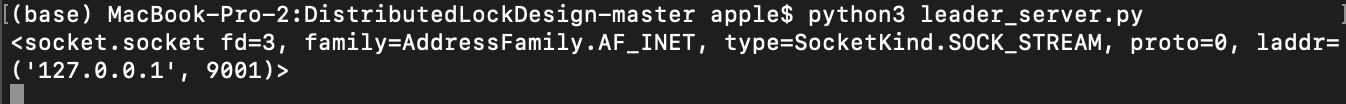
\includegraphics[width = 1\textwidth]{screenshot//leader_01.png}}
% \label{fig_process}
\end{figure}

Then, we start the follower server a and b. We set the port of follower server a to be 9002, b to be 9003. And they will get their ids: 2 and 3.

\begin{figure}[H]
\centerline{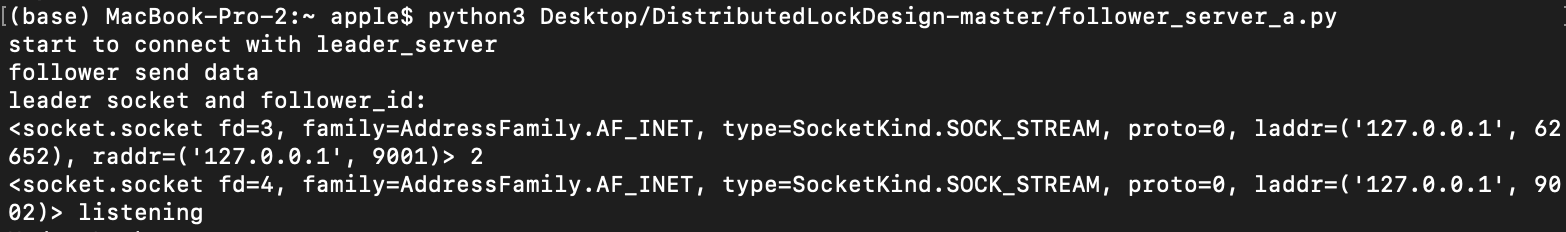
\includegraphics[width = 1\textwidth]{screenshot//follower_a_01.png}}
%\caption{Usage: put}
% \label{fig_process}
\end{figure}

\begin{figure}[H]
\centerline{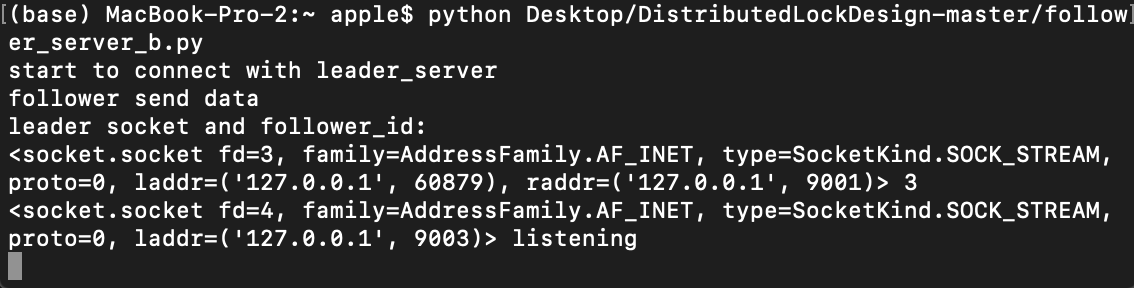
\includegraphics[width = 1\textwidth]{screenshot//follower_b_01.png}}
%\caption{Usage: put}
% \label{fig_process}
\end{figure}

And the leader server will connect to follower server a and b.

\begin{figure}[H]
\centerline{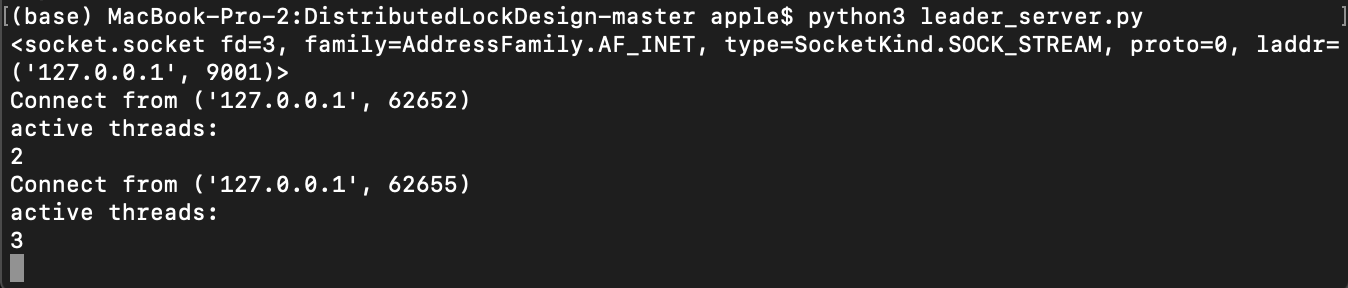
\includegraphics[width = 1\textwidth]{screenshot//leader_02.png}}
%\caption{Usage: read}
% \label{fig_process}
\end{figure}

Next, we start client a, and make it directly connect to leader server which means port 9001. It will get its ID:10001.

\begin{figure}[H]
\centerline{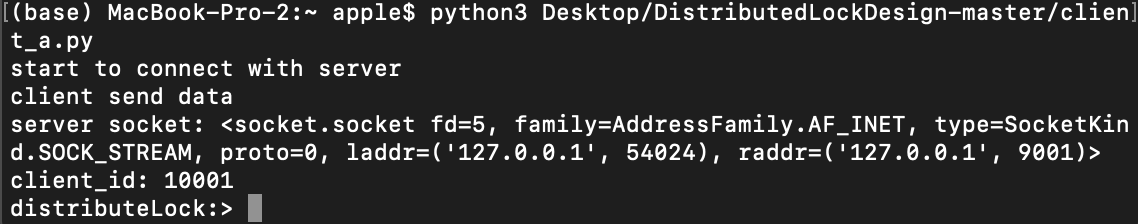
\includegraphics[width = 1\textwidth]{screenshot//client_01.png}}
%\caption{Usage: fetch}
% \label{fig_process}
\end{figure}

Then client a tried to preempt lock01.

\begin{figure}[H]
\centerline{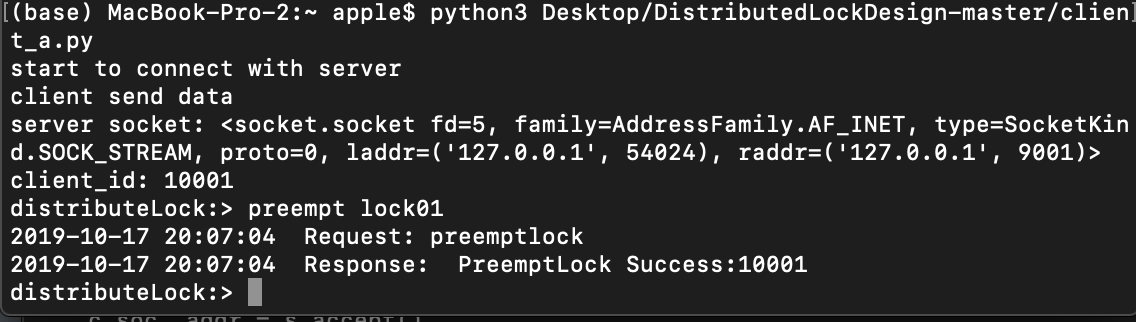
\includegraphics[width = 1\textwidth]{screenshot//client_02.png}}
%\caption{Usage: fetch}
% \label{fig_process}
\end{figure}

Leader server will check the lock list and give it a response. Also update the new state of lock01 and broadcast to all the follower servers.

\begin{figure}[H]
\centerline{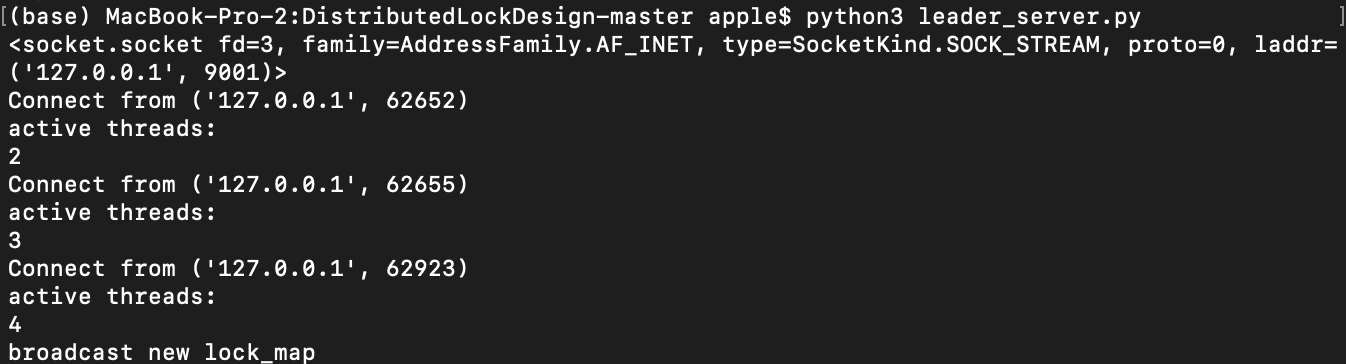
\includegraphics[width = 1\textwidth]{screenshot//leader_03.png}}
%\caption{Usage: recover}
% \label{fig_process}
\end{figure}


\begin{figure}[H]
\centerline{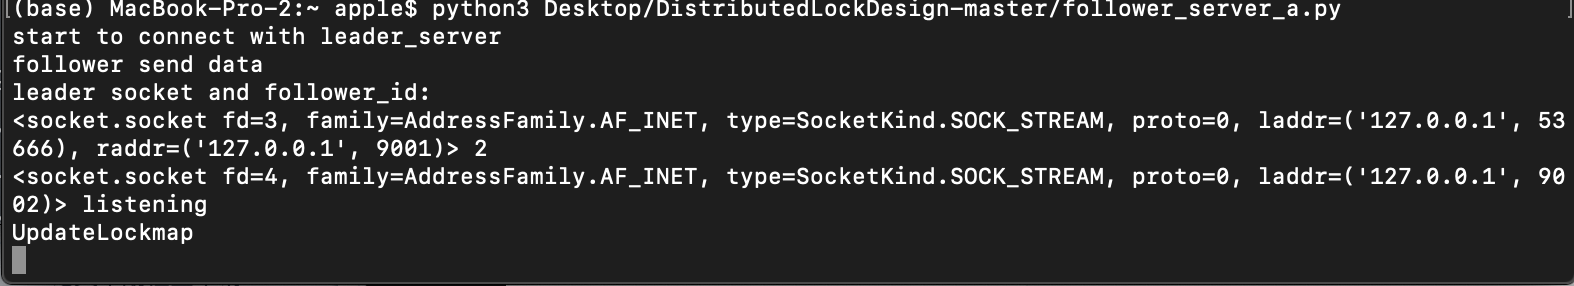
\includegraphics[width = 1\textwidth]{screenshot//follower_a_02.png}}
%\caption{Usage: recover}
% \label{fig_process}
\end{figure}

\begin{figure}[H]
\centerline{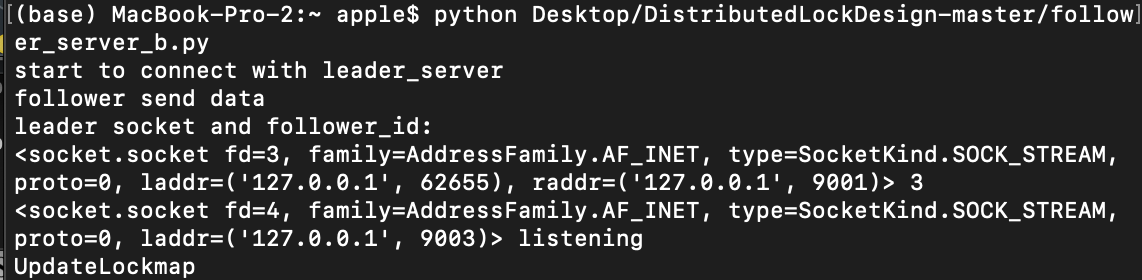
\includegraphics[width = 1\textwidth]{screenshot//follower_b_02.png}}
%\caption{Usage: recover}
% \label{fig_process}
\end{figure}


We start client b which is connected to follower server a. It will get its ID: 20001.

\begin{figure}[H]
\centerline{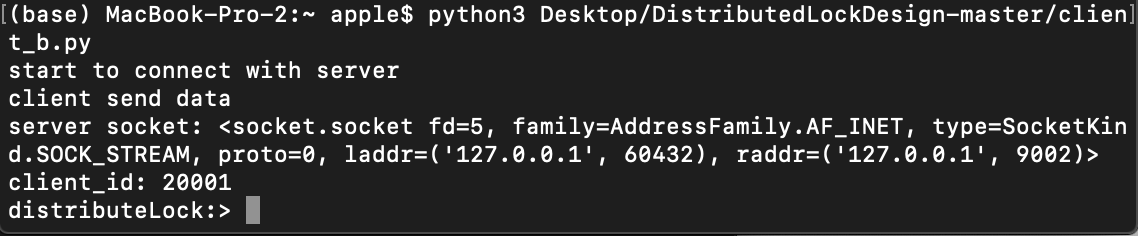
\includegraphics[width = 1\textwidth]{screenshot//client_03.png}}
%\caption{Usage: recover}
% \label{fig_process}
\end{figure}

\begin{figure}[H]
\centerline{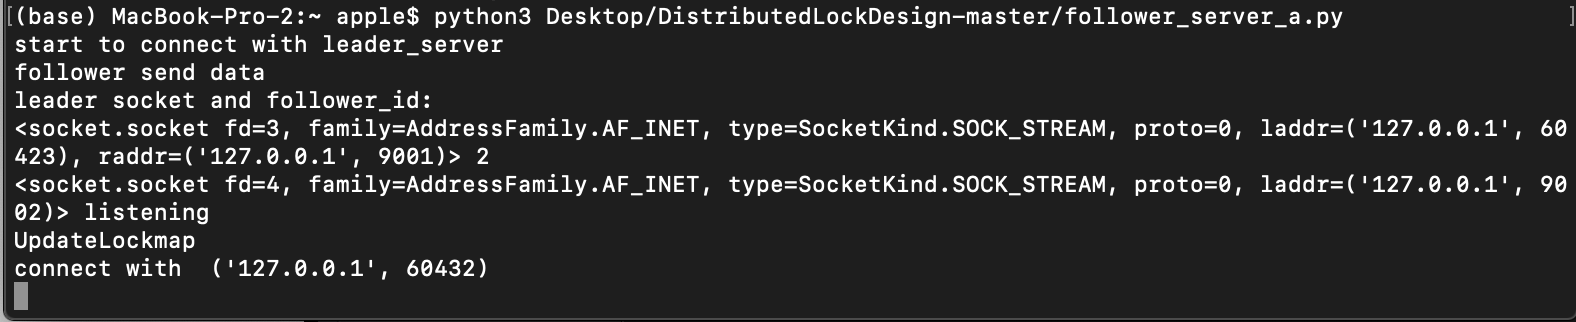
\includegraphics[width = 1\textwidth]{screenshot//follower_a_03.png}}
%\caption{Usage: quit}
% \label{fig_process}
\end{figure}

The client b check the lock01. The follower server a will tell it who owns lock01.

\begin{figure}[H]
\centerline{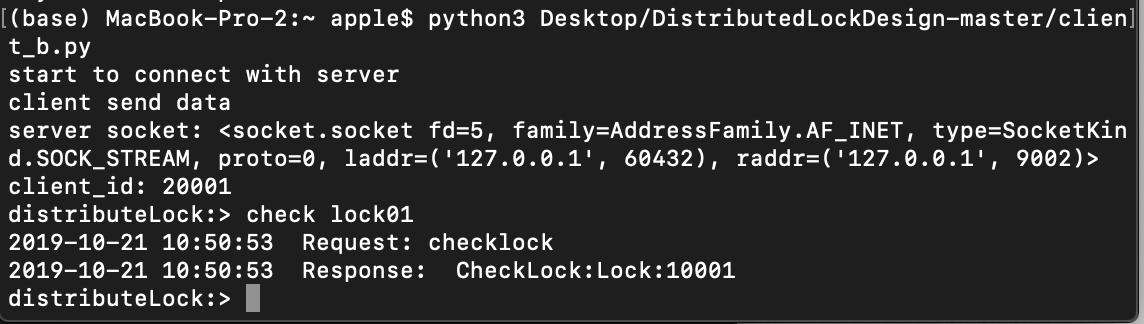
\includegraphics[width = 1\textwidth]{screenshot//client_04.png}}
%\caption{Usage: recover}
% \label{fig_process}
\end{figure}

The client b preempt the lock01. Obviously it will fail.

\begin{figure}[H]
\centerline{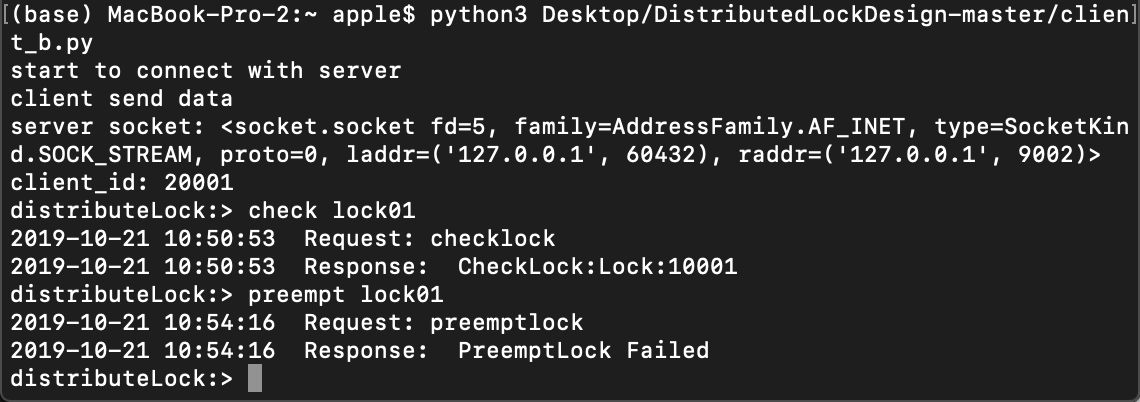
\includegraphics[width = 1\textwidth]{screenshot//client_05.png}}
%\caption{Usage: recover}
% \label{fig_process}
\end{figure}

Then client b preempt the lock02. Leader server will check the lock list and give it a response. Also update the new state of lock02 and broadcast to all the follower servers.

\begin{figure}[H]
\centerline{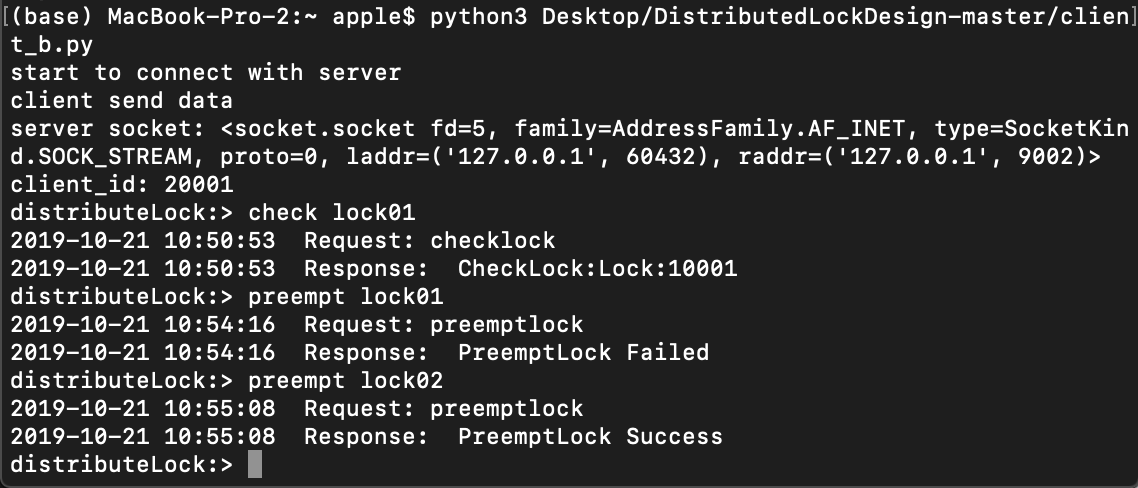
\includegraphics[width = 1\textwidth]{screenshot//client_06.png}}
%\caption{Usage: recover}
% \label{fig_process}
\end{figure}

\begin{figure}[H]
\centerline{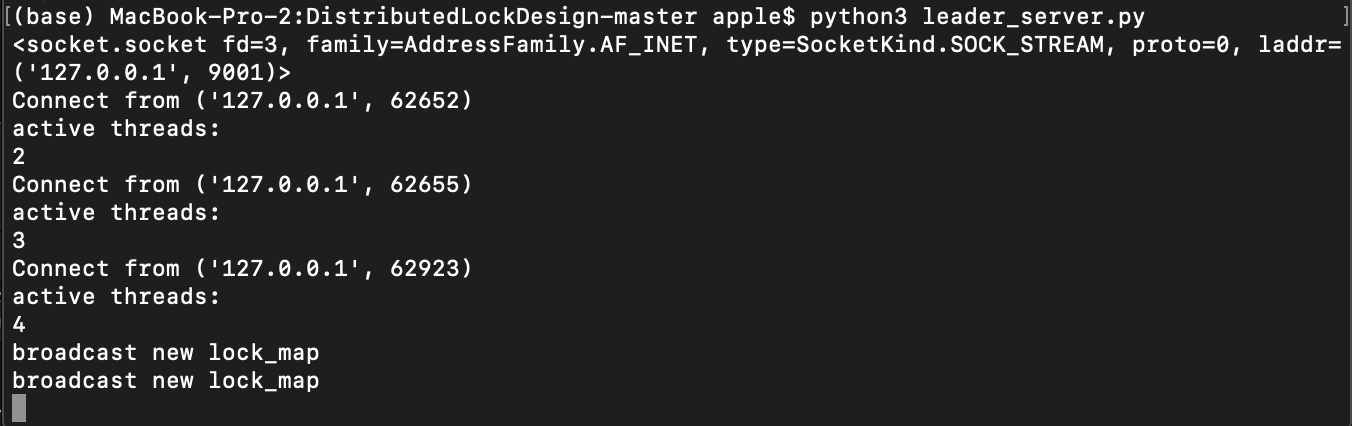
\includegraphics[width = 1\textwidth]{screenshot//leader_04.png}}
%\caption{Usage: recover}
% \label{fig_process}
\end{figure}

\begin{figure}[H]
\centerline{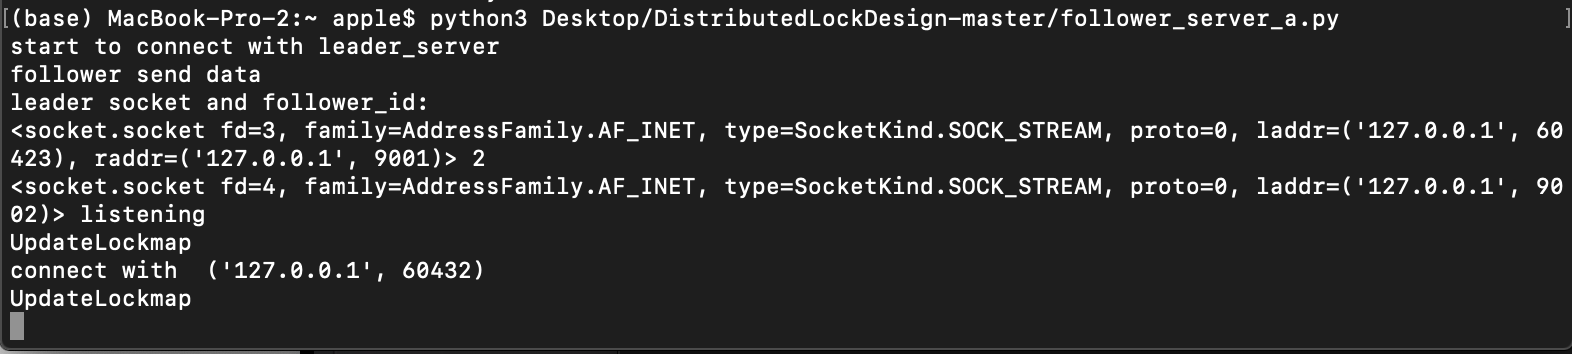
\includegraphics[width = 1\textwidth]{screenshot//follower_a_04.png}}
%\caption{Usage: recover}
% \label{fig_process}
\end{figure}

\begin{figure}[H]
\centerline{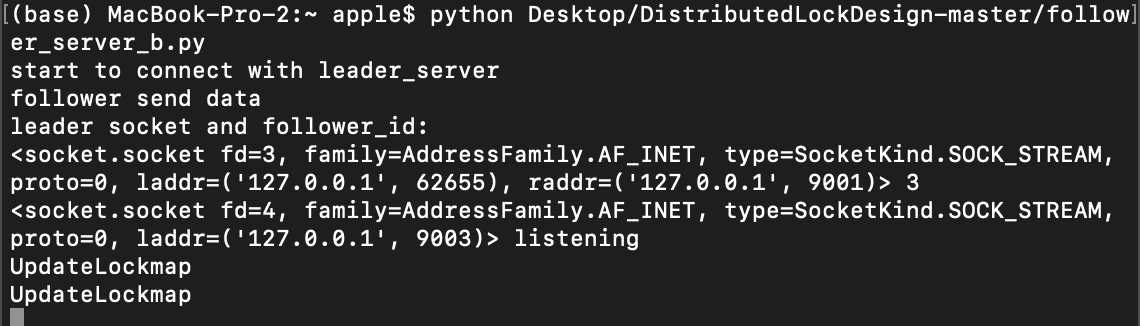
\includegraphics[width = 1\textwidth]{screenshot//follower_b_03.png}}
%\caption{Usage: recover}
% \label{fig_process}
\end{figure}



Start client c which is connected to follower server b. It will get its ID: 30001

\begin{figure}[H]
\centerline{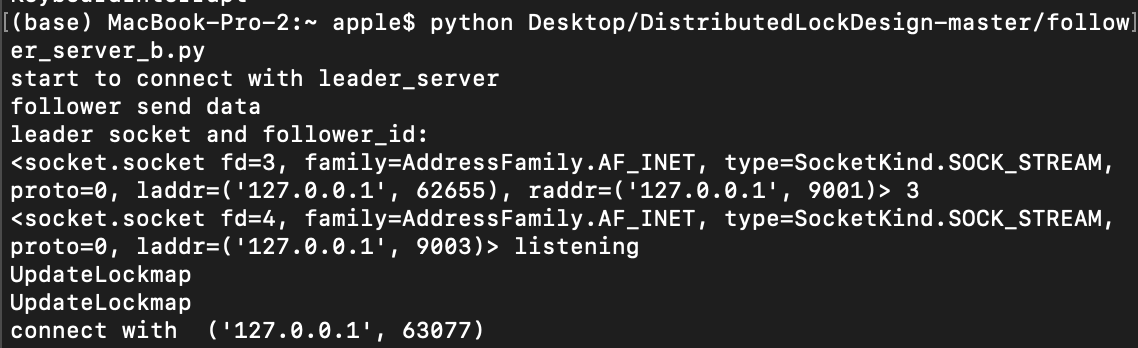
\includegraphics[width = 1\textwidth]{screenshot//follower_b_04.png}}
%\caption{Usage: recover}
% \label{fig_process}
\end{figure}

\begin{figure}[H]
\centerline{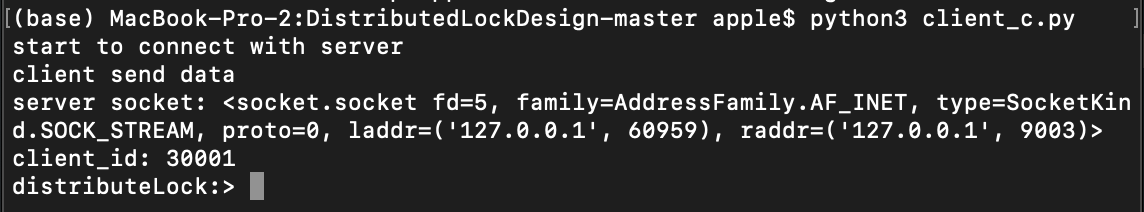
\includegraphics[width = 1\textwidth]{screenshot//client_07.png}}
%\caption{Usage: recover}
% \label{fig_process}
\end{figure}


Client c preempt lock 02. It will fail.
\begin{figure}[H]
\centerline{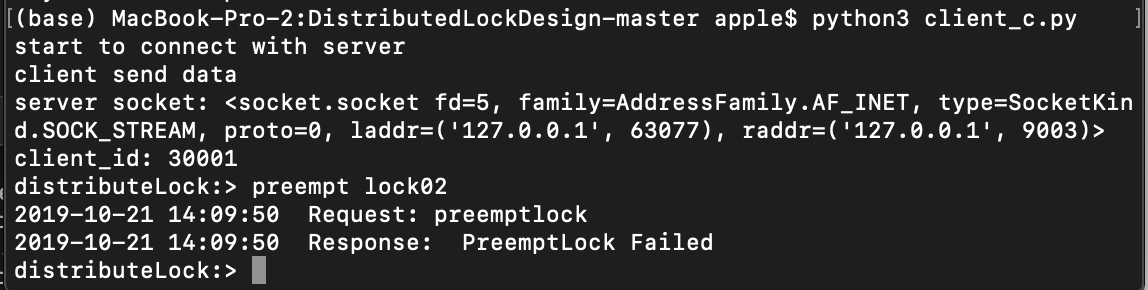
\includegraphics[width = 1\textwidth]{screenshot//client_08.png}}
%\caption{Usage: recover}
% \label{fig_process}
\end{figure}

Then client b release the lock02. Leader server will check the lock list and remove lock02 from the list. Also update the new state of lock02 and broadcast to all the follower servers.
\begin{figure}[H]
\centerline{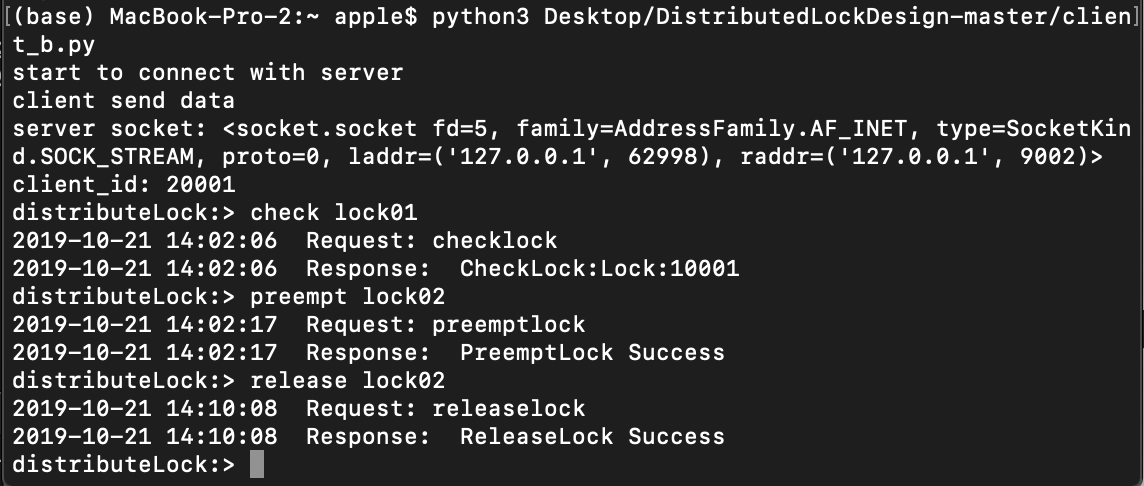
\includegraphics[width = 1\textwidth]{screenshot//client_09.png}}
%\caption{Usage: recover}
% \label{fig_process}
\end{figure}

\begin{figure}[H]
\centerline{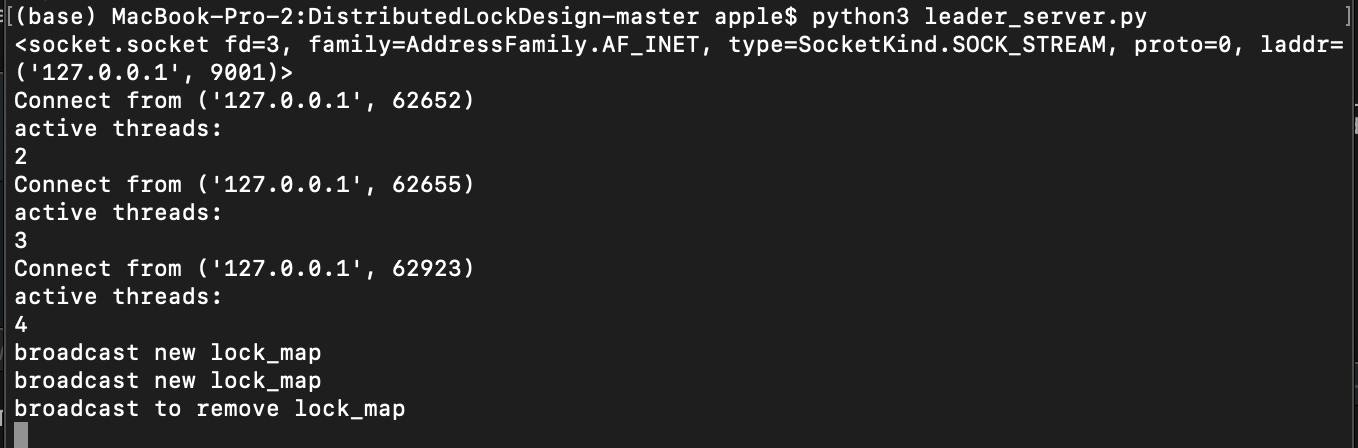
\includegraphics[width = 1\textwidth]{screenshot//leader_05.png}}
%\caption{Usage: recover}
% \label{fig_process}
\end{figure}

\begin{figure}[H]
\centerline{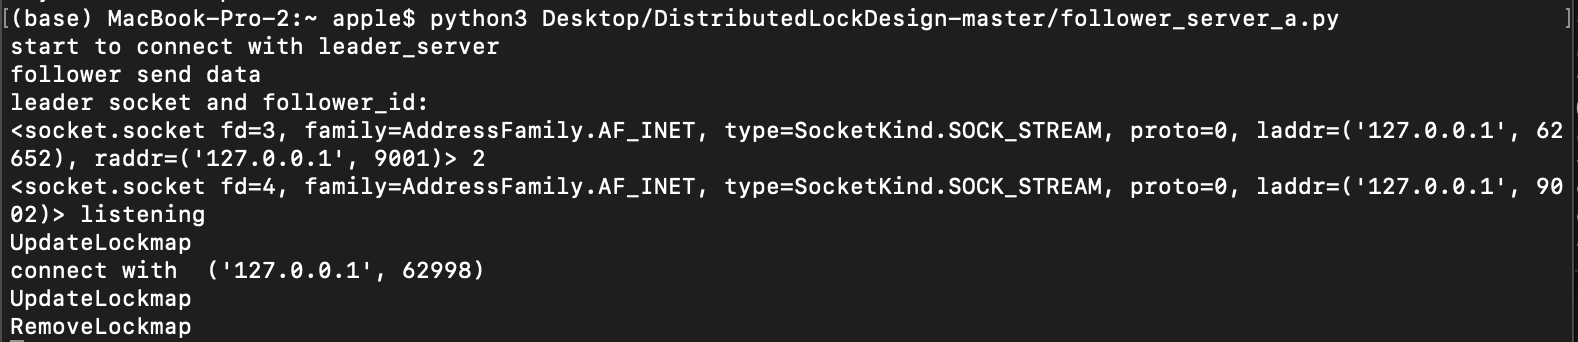
\includegraphics[width = 1\textwidth]{screenshot//follower_a_05.png}}
%\caption{Usage: recover}
% \label{fig_process}
\end{figure}

\begin{figure}[H]
\centerline{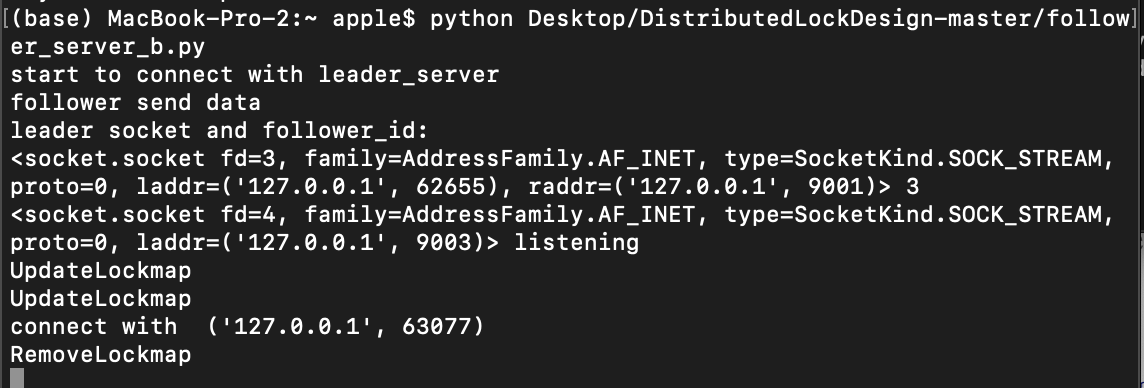
\includegraphics[width = 1\textwidth]{screenshot//follower_b_05.png}}
%\caption{Usage: recover}
% \label{fig_process}
\end{figure}

Now client c and successfully preempt lock02. And client a will know the owner of lock02 if it check lock02.

\begin{figure}[H]
\centerline{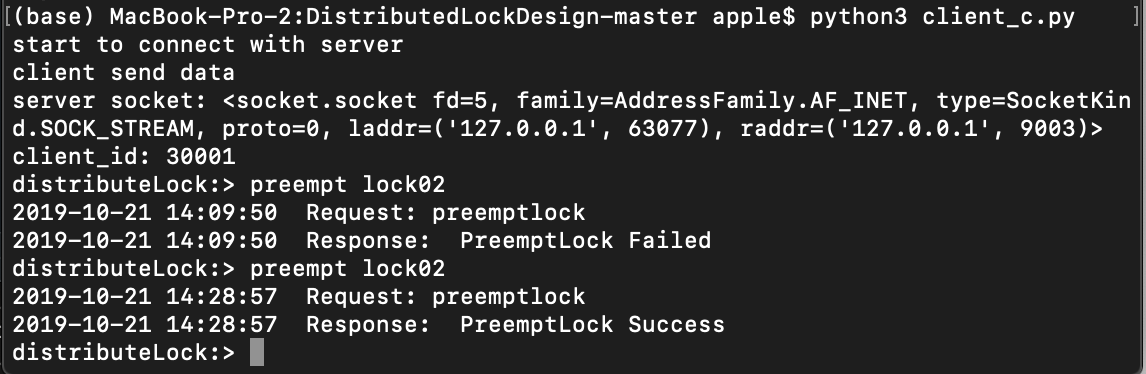
\includegraphics[width = 1\textwidth]{screenshot//client_10.png}}
%\caption{Usage: recover}
% \label{fig_process}
\end{figure}

\begin{figure}[H]
\centerline{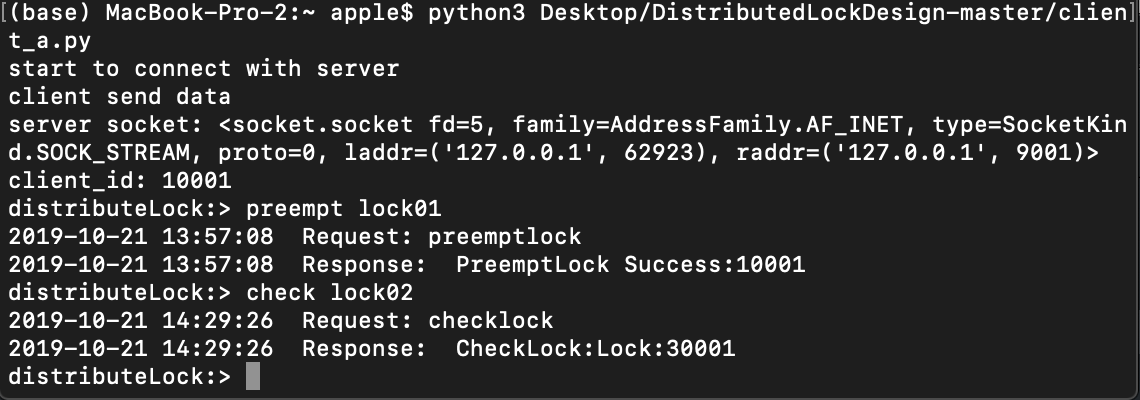
\includegraphics[width = 1\textwidth]{screenshot//client_11.png}}
%\caption{Usage: recover}
% \label{fig_process}
\end{figure}
% \begin{figure}[h]
% \centerline{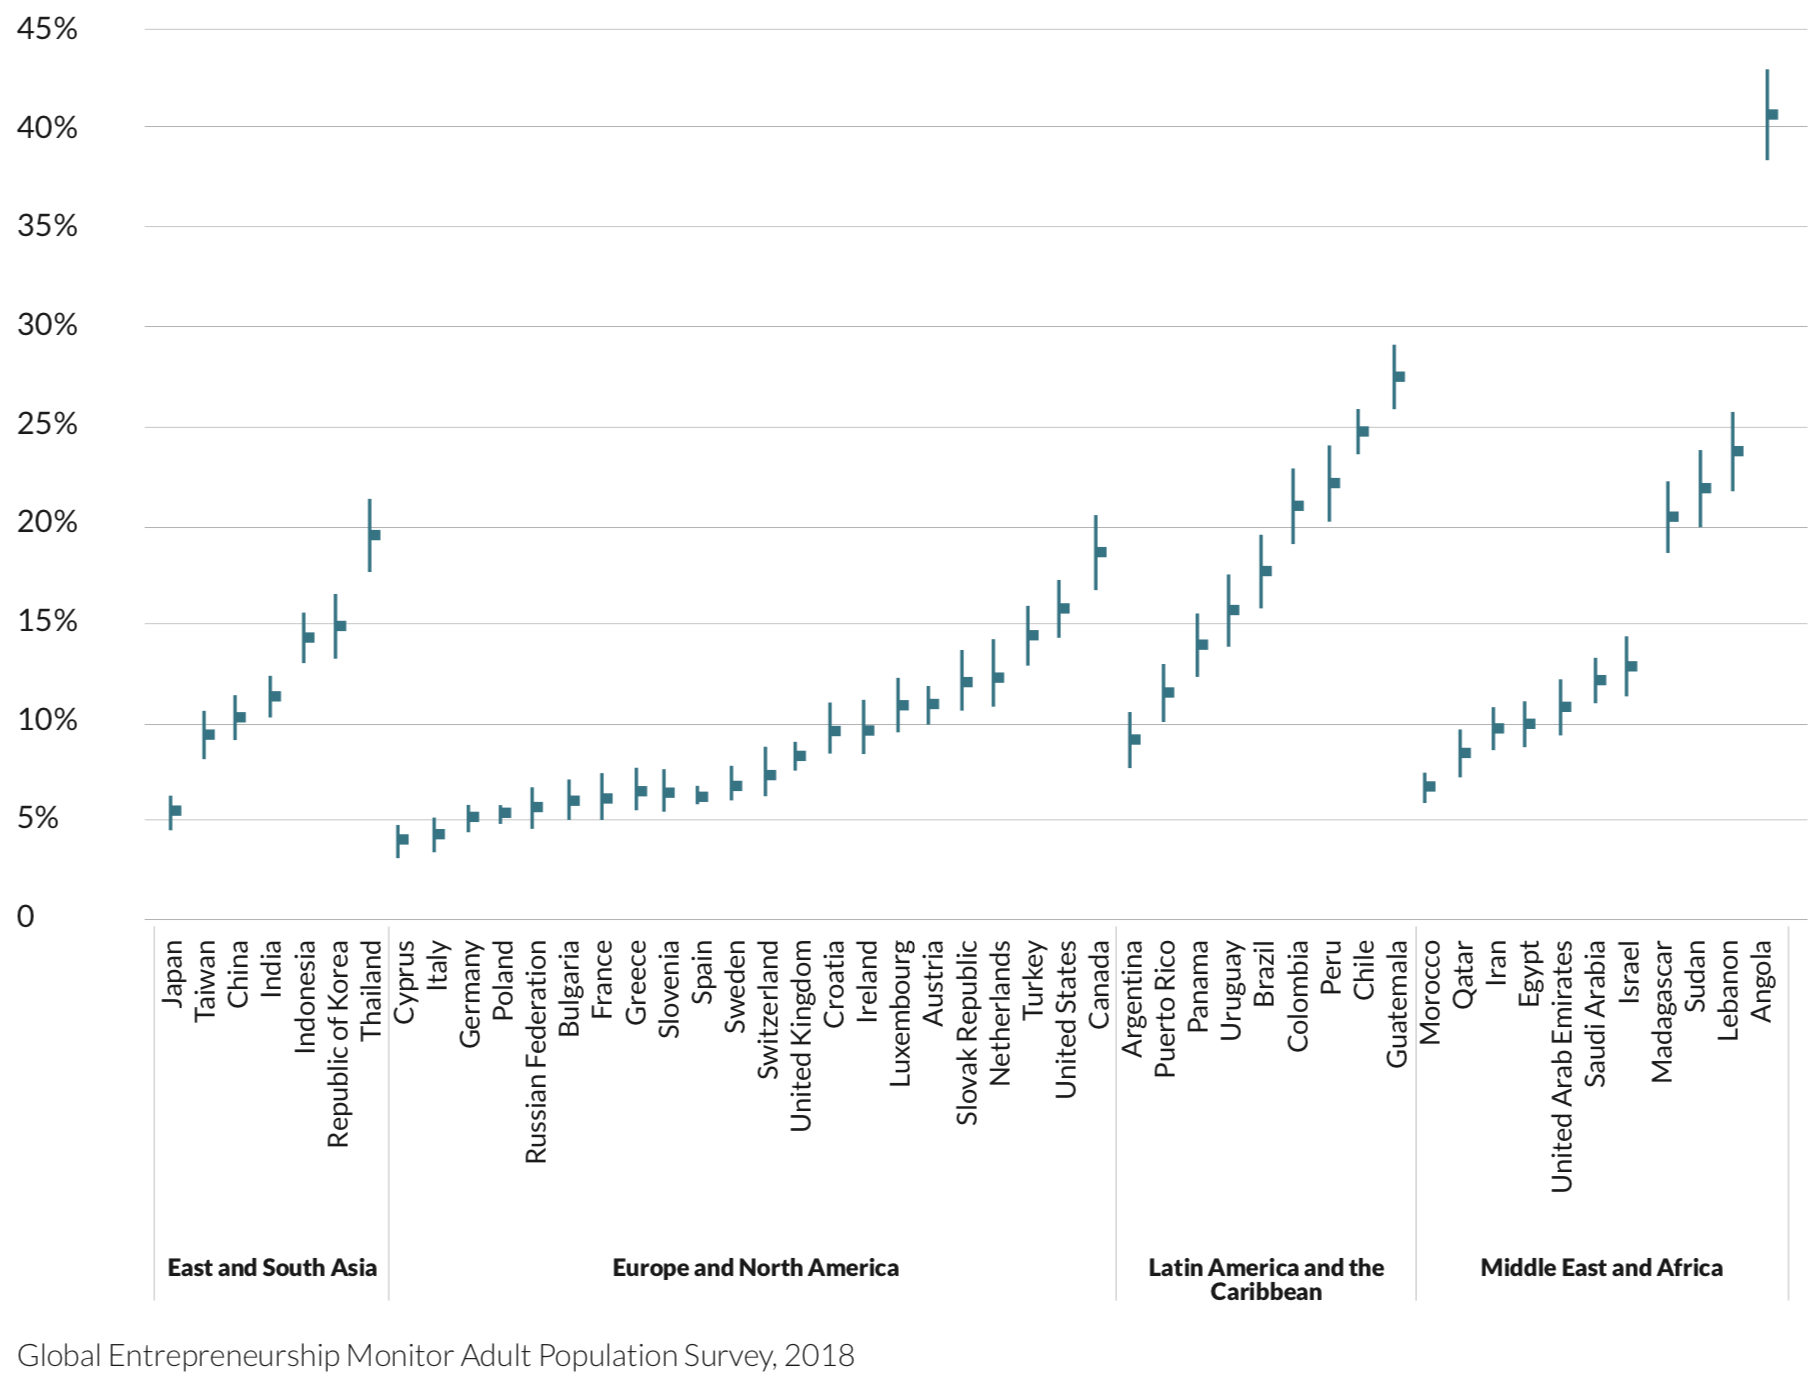
\includegraphics[width = 1\textwidth]{screenshot//2_2.png}}
% \caption{Total early-stage Entrepreneurial Activity (TEA) Rates among Adults (ages 18-64) in 487 Economies, in Four Geographic Regions}
% \label{fig_TEA_global}
% \end{figure}

% \section{Pod}
% \subsection{1 Pod with 1 Container}
%
% We can see after creating pod1 by pod1.yaml, we can execute any command by kubectl exec -it pod1 -- command.
%
% \begin{figure}[H]
% \centerline{\includegraphics[width = 0.7\textwidth]{screenshot//1.png}}
% \caption{1 Pod with 1 Container}
% % \label{fig_1pod1container}
% \end{figure}
%
% \subsection{1 Pod with 2 Containers}
%
% We can see after we change index.html in container ct-debian, we can also see the change in container ct-nginx.
%
% \begin{figure}[H]
% \centerline{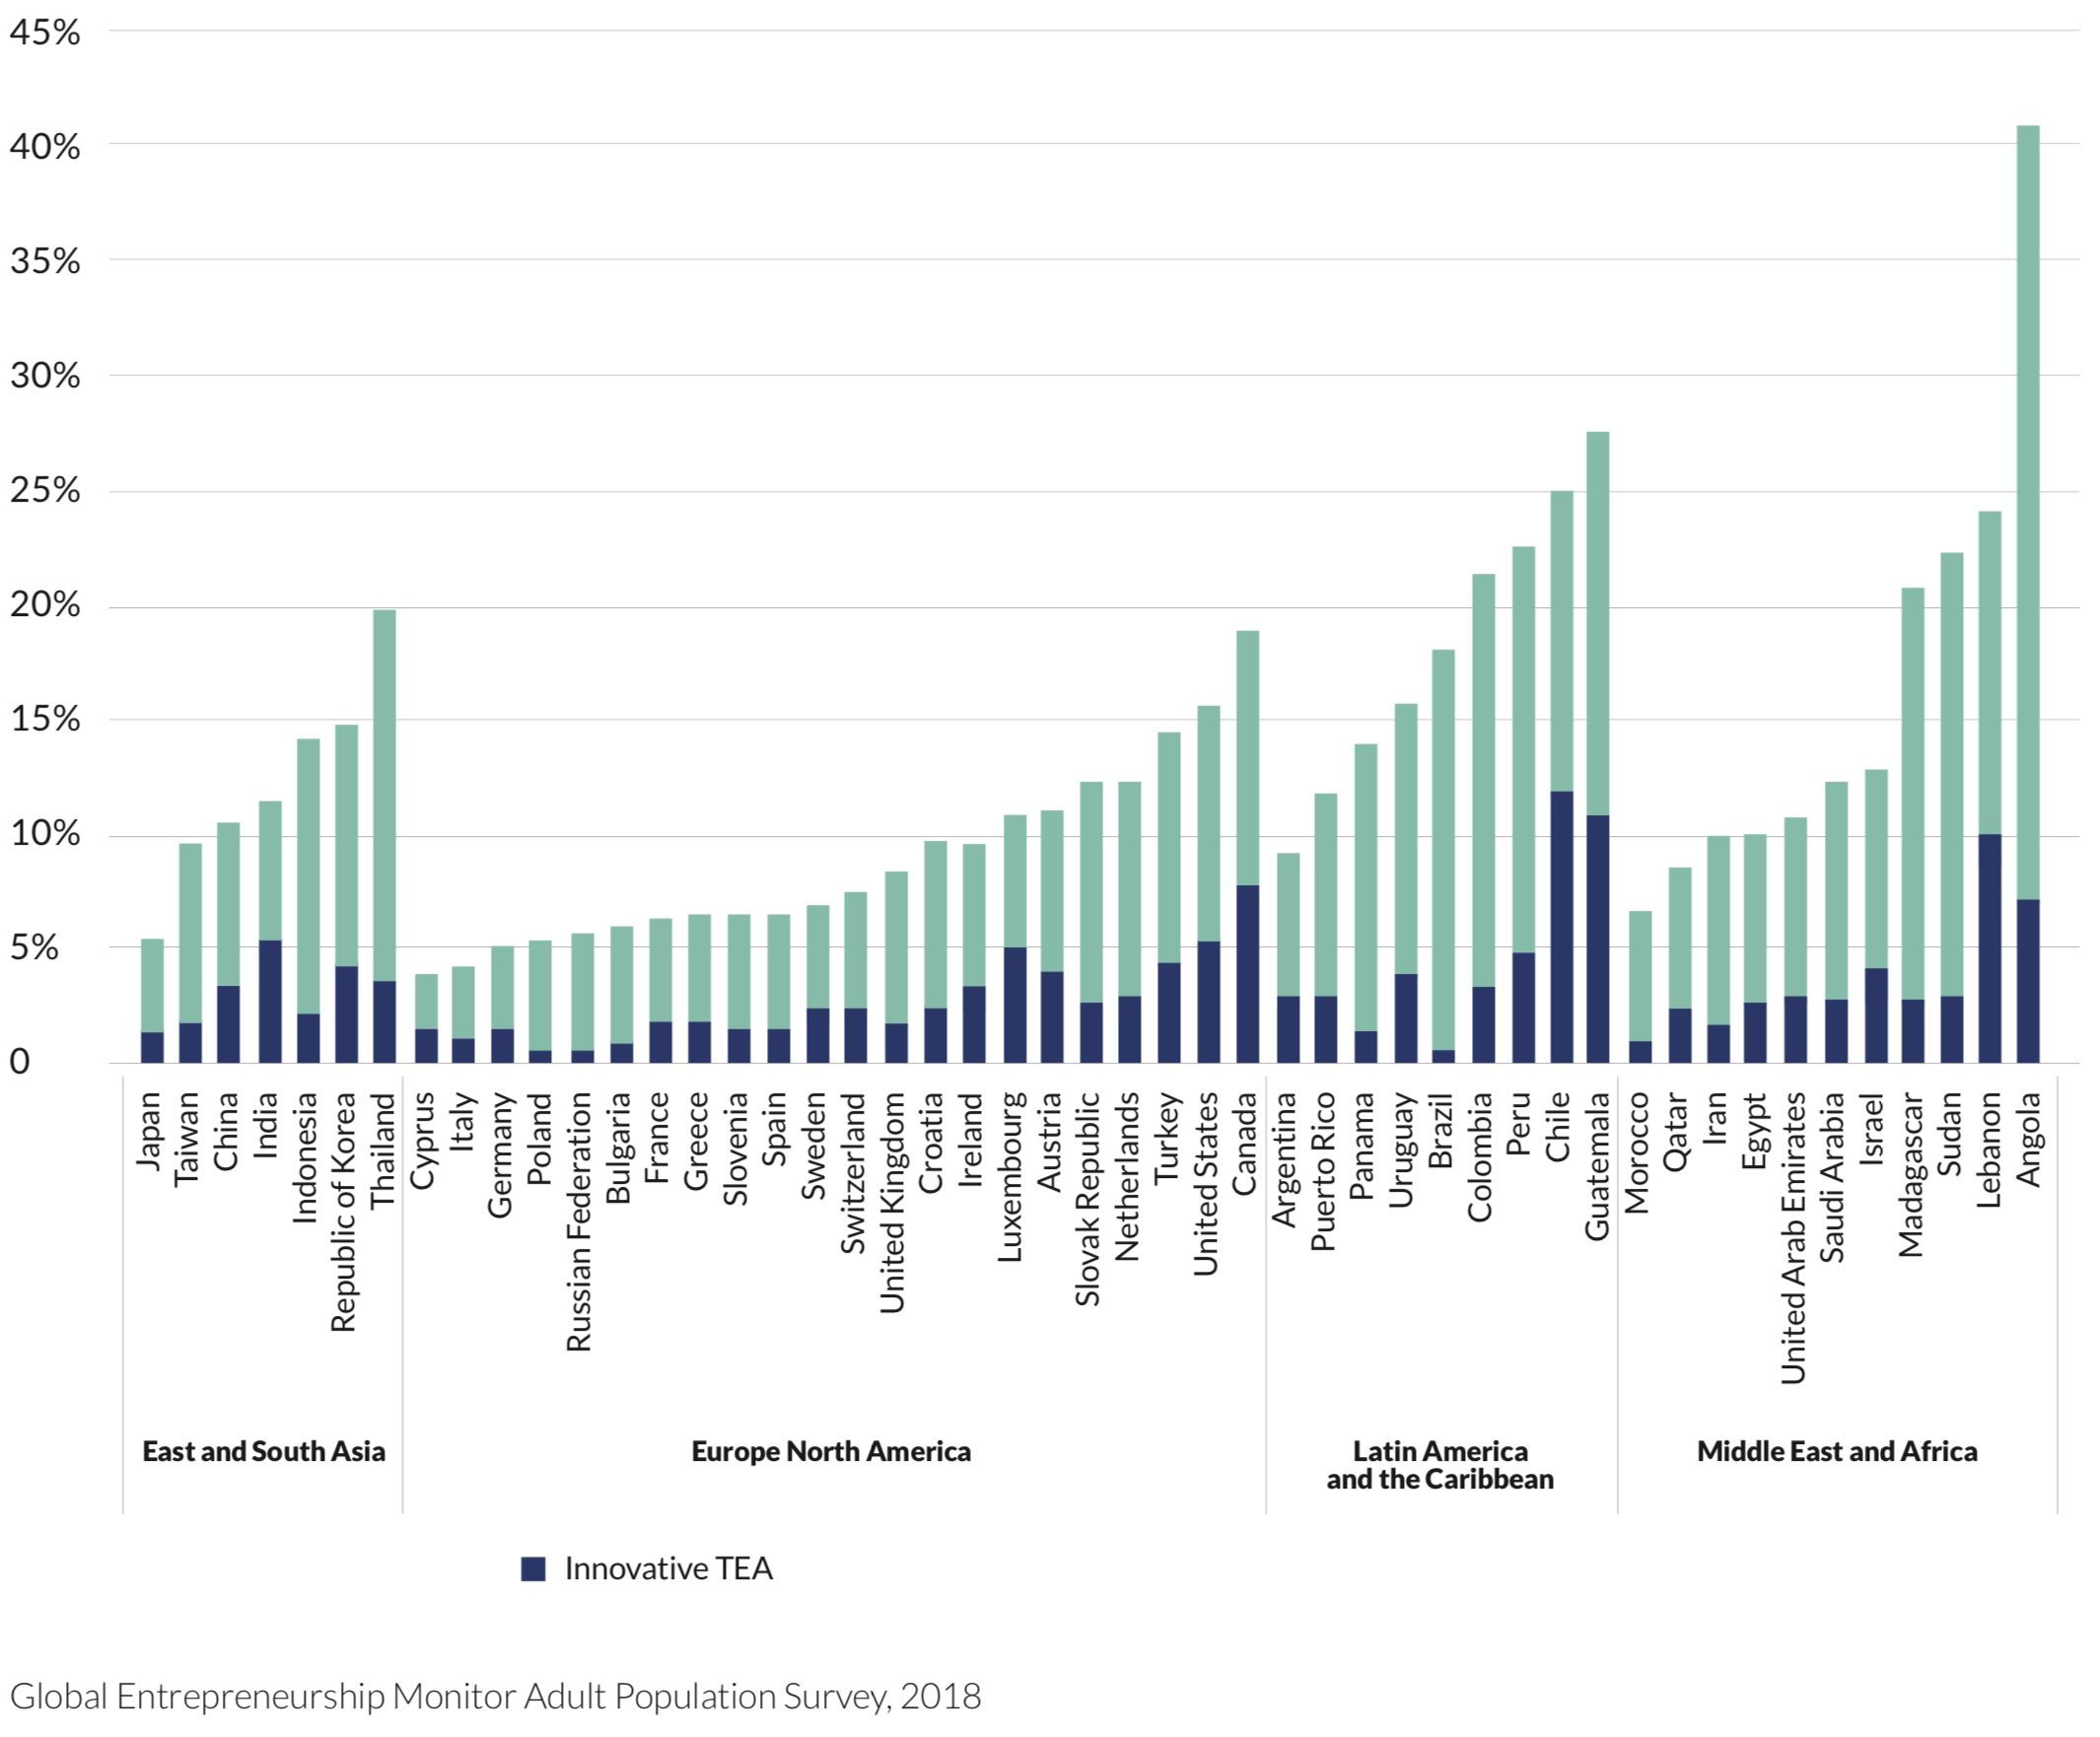
\includegraphics[width = 0.7\textwidth]{screenshot//2_1.png}}
% \caption{1 Pod with 2 Container}
% % \label{fig_1pod1container}
% \end{figure}






\end{document}
